\tikzset{every picture/.style={line width=0.75pt}} %set default line width to 0.75pt        

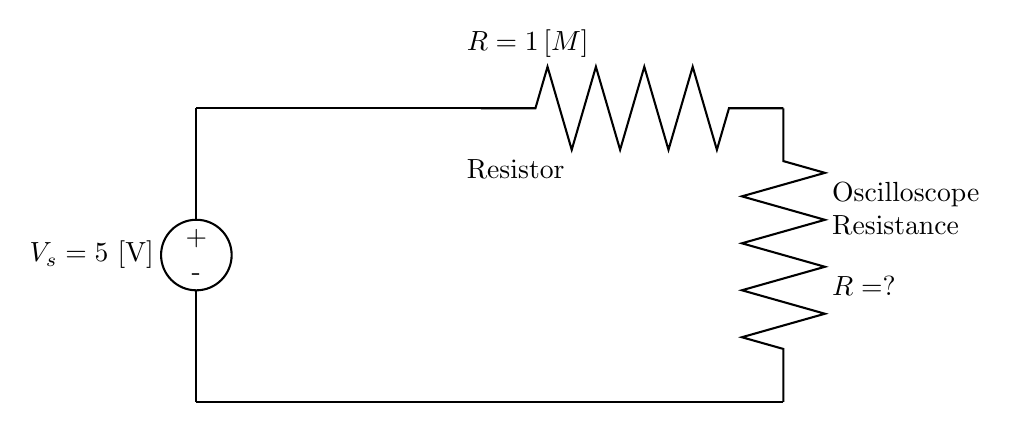
\begin{tikzpicture}[x=0.75pt,y=0.75pt,yscale=-1,xscale=1]
%uncomment if require: \path (0,642); %set diagram left start at 0, and has height of 642

%Shape: Circle [id:dp1293335169248646] 
\draw   (100,140) .. controls (100,130.61) and (107.61,123) .. (117,123) .. controls (126.39,123) and (134,130.61) .. (134,140) .. controls (134,149.39) and (126.39,157) .. (117,157) .. controls (107.61,157) and (100,149.39) .. (100,140) -- cycle ;
%Straight Lines [id:da8573659817175756] 
\draw    (117,69.29) -- (117,123) ;
%Straight Lines [id:da09626430681968268] 
\draw    (117,157) -- (117,210.71) ;
%Straight Lines [id:da19138905725146715] 
\draw    (258.42,69.29) -- (117,69.29) ;
%Straight Lines [id:da9383173165485992] 
\draw    (258.42,210.71) -- (117,210.71) ;
%Straight Lines [id:da51555500958681] 
\draw    (399.84,210.71) -- (258.42,210.71) ;
%Shape: Resistor [id:dp8459054998005646] 
\draw   (254.13,69.29) -- (280.36,69.29) -- (286.19,49.29) -- (297.85,89.29) -- (309.5,49.29) -- (321.16,89.29) -- (332.82,49.29) -- (344.47,89.29) -- (356.13,49.29) -- (367.79,89.29) -- (373.61,69.29) -- (399.84,69.29) ;
%Shape: Resistor [id:dp3577155889138255] 
\draw   (399.84,69.29) -- (399.84,94.75) -- (419.84,100.4) -- (379.84,111.72) -- (419.84,123.03) -- (379.84,134.34) -- (419.84,145.66) -- (379.84,156.97) -- (419.84,168.28) -- (379.84,179.6) -- (399.84,185.25) -- (399.84,210.71) ;

% Text Node
\draw (117,126) node [anchor=north] [inner sep=0.75pt]   [align=left] {\begin{minipage}[lt]{8.68pt}\setlength\topsep{0pt}
\begin{center}
+
\end{center}

\end{minipage}};
% Text Node
\draw (117,154) node [anchor=south] [inner sep=0.75pt]   [align=left] {\begin{minipage}[lt]{8.67pt}\setlength\topsep{0pt}
\begin{center}
\mbox{-}
\end{center}

\end{minipage}};
% Text Node
\draw (98,140) node [anchor=east] [inner sep=0.75pt]   [align=left] {$\displaystyle V_{s} =5$ [V]};
% Text Node
\draw (295.85,92.29) node [anchor=north east] [inner sep=0.75pt]   [align=left] {Resistor};
% Text Node
\draw (307.5,46.29) node [anchor=south east] [inner sep=0.75pt]   [align=left] {$\displaystyle R=1\left[\text{M} \si{\ohm}\right]$};
% Text Node
\draw (421.84,103.4) node [anchor=north west][inner sep=0.75pt]   [align=left] {Oscilloscope\\Resistance};
% Text Node
\draw (421.84,148.66) node [anchor=north west][inner sep=0.75pt]   [align=left] {$\displaystyle R=?$};


\end{tikzpicture}
